\documentclass[crop,tikz,10pt]{standalone}
\usepackage{tikz}
	\usetikzlibrary{shapes}
	\usetikzlibrary{automata}
	\usetikzlibrary{arrows}
	\usetikzlibrary{backgrounds}
	\usetikzlibrary{calc}
	\usetikzlibrary{positioning}
	\usetikzlibrary{patterns}
	\usetikzlibrary{decorations.pathmorphing}
	\usetikzlibrary{decorations.pathreplacing}

\usepackage[scaled]{helvet}
\renewcommand{\familydefault}{\sfdefault}

\usepackage{siunitx}
\usepackage{booktabs}

\input{../../../../resources/latex/_symbols.qmd}

\begin{document}


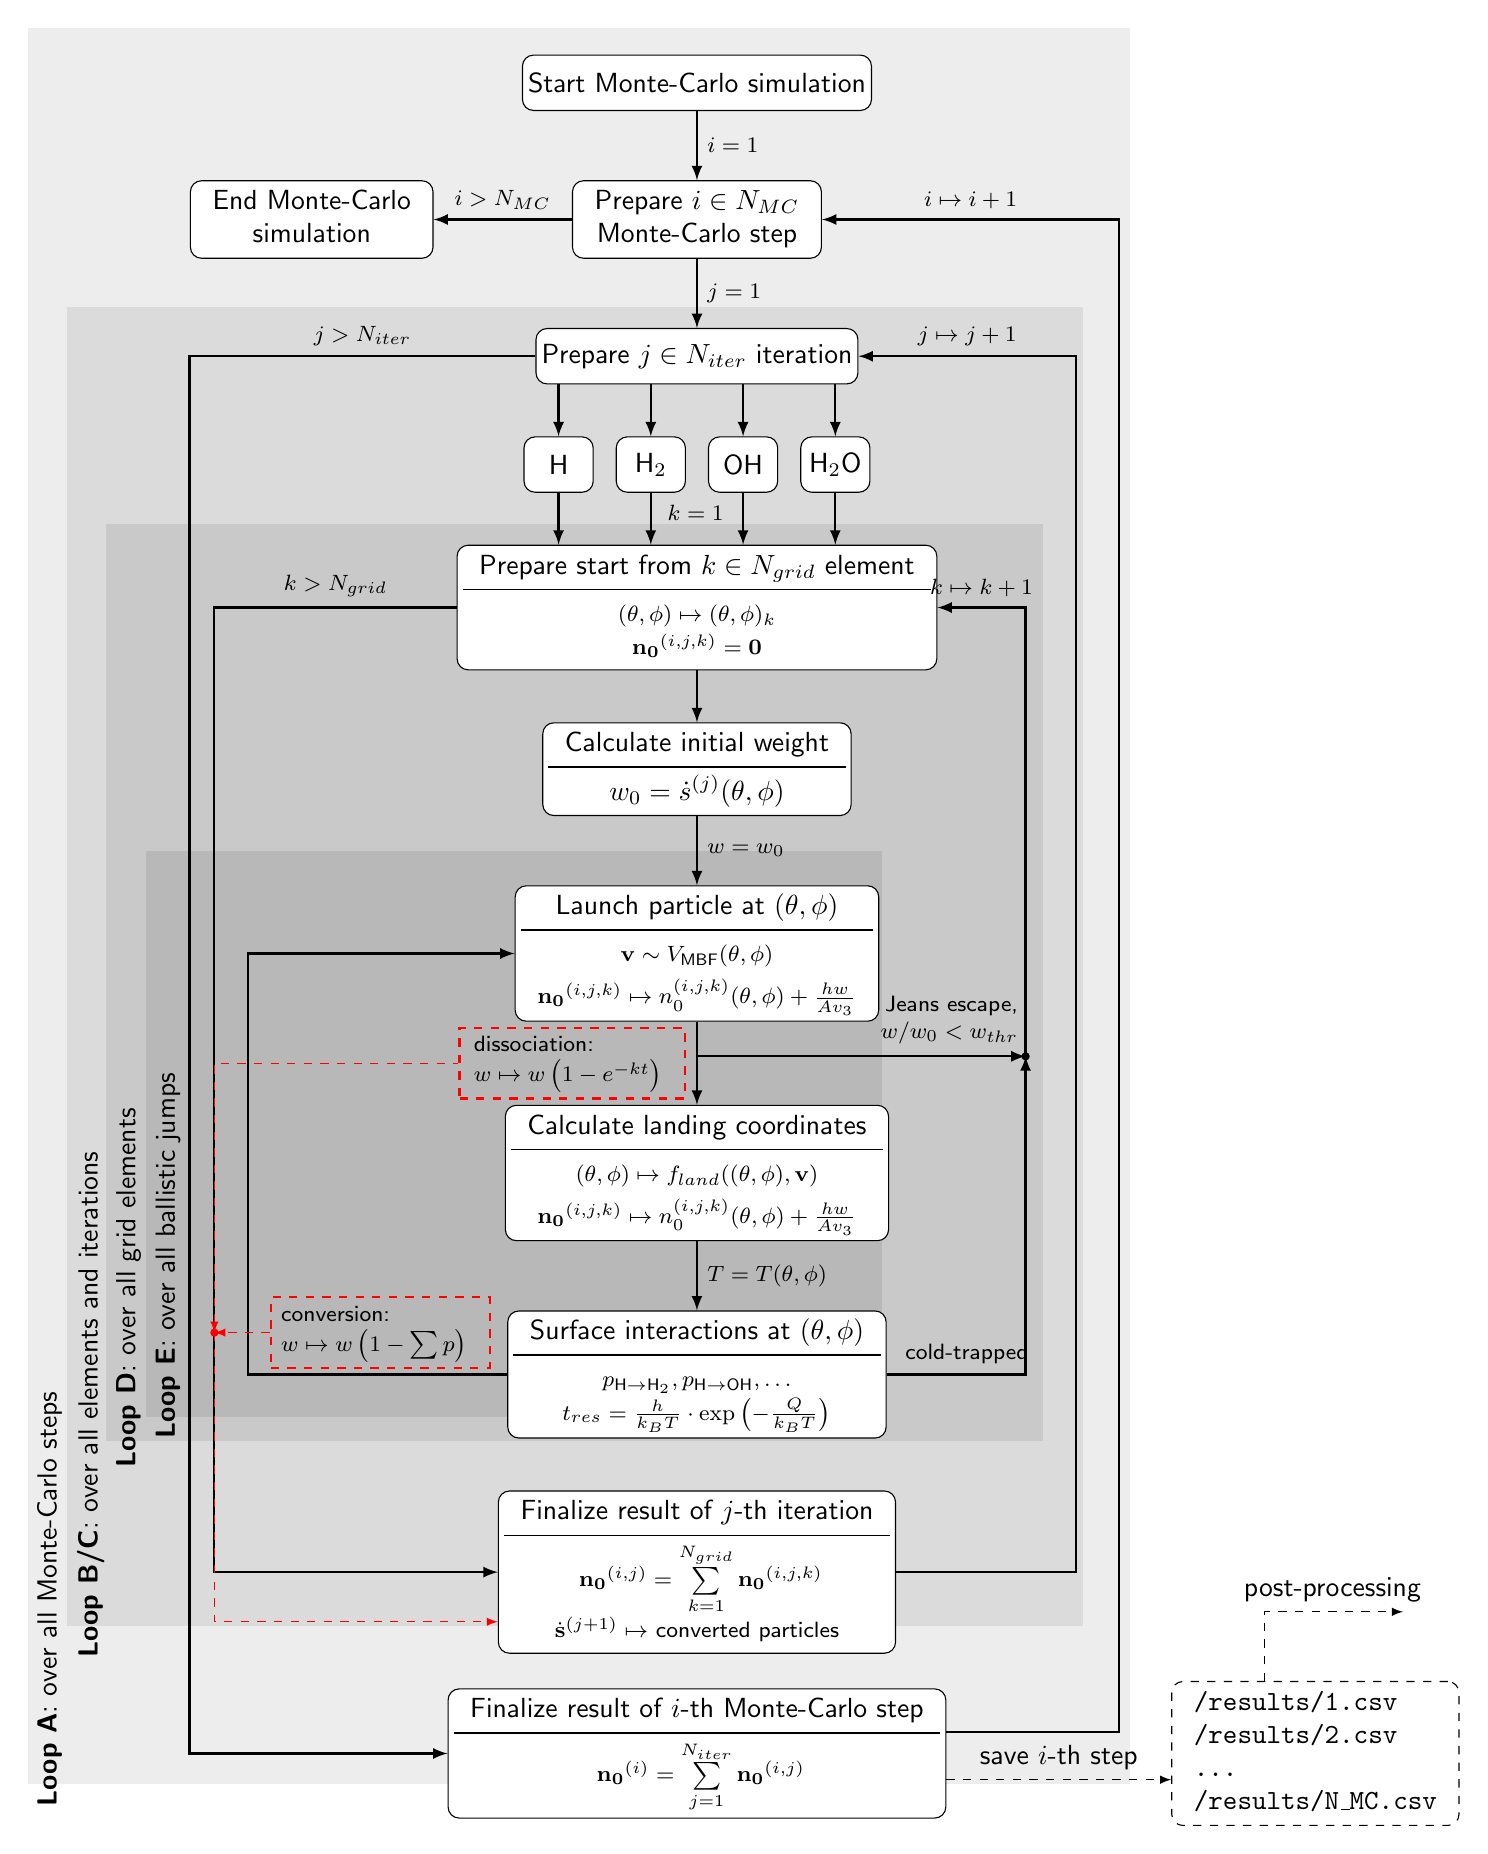
\begin{tikzpicture}[
    main/.style={draw, rounded corners=4pt, inner sep=2pt, minimum size=20pt, minimum width=25pt, fill=white},
    sub/.style={draw, rounded corners=4pt, inner sep=2pt},
]    
    %% VARIABLES
    \def\h{25pt};

    %% BACKGROUNDS
    \fill[black!7!white] (-8.5,0.7) rectangle +(14.0,-22.3)node[at start, below left, rotate=90, black, xshift=-172mm]{\textbf{Loop A}: over all Monte-Carlo steps};
    \fill[black!14!white] (-8.0,-2.85) rectangle +(12.9,-16.75)node[at start, below left, rotate=90, black, xshift=-106mm]{\textbf{Loop B/C}: over all elements and iterations};
    \fill[black!21!white] (-7.5,-5.6) rectangle +(11.9,-11.65)node[at start, below left, rotate=90, black, xshift=-73mm]{\textbf{Loop D}: over all grid elements};
    \fill[black!28!white] (-7,-9.75) rectangle +(9.35,-7.2)node[at start, below left, rotate=90, black, xshift=-27mm]{\textbf{Loop E}: over all ballistic jumps};

    %% NODES
    % steps
    \node[main] (START) at (0,0) {Start Monte-Carlo simulation};
    % \node[draw, minimum width=18*\h, minimum height=28*\h, below=\h of START] (MC) {};
    \node[main, below=\h of START] (MCSTEP) {\begin{tabular}{c}Prepare $i \in N_{MC}$\\Monte-Carlo step\end{tabular}};

    % iteration
    % \node[draw, minimum width=16*\h, minimum height=24*\h, below=\h of MCSTEP] {};
    \node[main, below=\h of MCSTEP] (ITERSTEP) {Prepare $j \in N_{iter}$ iteration};
    \node[main, below=0.75*\h of ITERSTEP, xshift=-2*\h] (H) {H};
    \node[main, below=0.75*\h of ITERSTEP, xshift=-0.6667*\h] (H2) {H$_2$};
    \node[main, below=0.75*\h of ITERSTEP, xshift= 0.6667*\h] (OH) {OH};
    \node[main, below=0.75*\h of ITERSTEP, xshift= 2*\h] (H2O) {H$_2$O};

    % grid
    % \node[draw, minimum width=14*\h, minimum height=16*\h, below=0.5*\h of H, xshift=2*\h] (GRIDLOOP) {};
    \node[main, below=0.75*\h of H, xshift=2*\h] (GRIDSTART) {\begin{tabular}{c}Prepare start from $k \in N_{grid}$ element\\\midrule \footnotesize{$(\theta, \phi) \mapsto (\theta, \phi)_k$}\\\footnotesize{$\mathbf{n_0}^{(i,j,k)} = \mathbf{0}$}\end{tabular}};
    \node[main, below=0.75*\h of GRIDSTART] (W0) {\begin{tabular}{c}Calculate initial weight\\\midrule $w_0 = \dot{s}^{(j)}(\theta, \phi)$\end{tabular}};
    \node[main, below=\h of W0] (LAUNCH) {\begin{tabular}{c}Launch particle at $(\theta, \phi)$\\\midrule\footnotesize{$\mathbf{v} \sim V_\text{MBF}(\theta, \phi)$}\\[1mm]\footnotesize{$\mathbf{n_0}^{(i,j,k)} \mapsto n_0^{(i,j,k)}(\theta, \phi) + \frac{hw}{Av_3}$}\end{tabular}};
    \node[main, below=1.2*\h of LAUNCH] (LAND) {\begin{tabular}{c}Calculate landing coordinates\\\midrule\footnotesize{$(\theta, \phi) \mapsto f_{land}((\theta, \phi), \mathbf{v})$}\\[1mm]\footnotesize{$\mathbf{n_0}^{(i,j,k)} \mapsto n_0^{(i,j,k)}(\theta, \phi) + \frac{hw}{Av_3}$}\end{tabular}};
    \node[main, below=\h of LAND] (SURF) {\begin{tabular}{c}Surface interactions at $(\theta, \phi)$\\\midrule\footnotesize{$p_{\text{H}\rightarrow\text{H}_2}, p_{\text{H}\rightarrow\text{OH}}, \dots$}\\\footnotesize{$t_{res} = \frac{h}{k_B T}\cdot\exp\left(-\frac{Q}{k_BT}\right)$}\end{tabular}};
    \node[main, below=0.75*\h of SURF] (GRIDEND) {\begin{tabular}{c}Finalize result of $j$-th iteration\\\midrule\footnotesize{ $\mathbf{n_0}^{(i, j)} = \sum\limits_{k=1}^{N_{grid}} \mathbf{n_0}^{(i, j, k)}$}\\\footnotesize{$\dot{\mathbf{s}}^{(j+1)} \mapsto$ converted particles}\end{tabular}};

    % iteration continued
    \node[main, below=0.5*\h of GRIDEND] (ITEREND) {\begin{tabular}{c}Finalize result of $i$-th Monte-Carlo step\\\midrule\footnotesize{ $\mathbf{n_0}^{(i)} = \sum\limits_{j=1}^{N_{iter}} \mathbf{n_0}^{(i, j)}$}\end{tabular}};

    % steps continued
    \node[main, left=2*\h of MCSTEP] (MCEDND) {\begin{tabular}{c}End Monte-Carlo\\simulation\end{tabular}};

    % postprocessing
    \node[main, dashed, right=3.25*\h of ITEREND] (SAVE) {\begin{tabular}{l}\texttt{/results/1.csv}\\\texttt{/results/2.csv}\\\texttt{...}\\\texttt{/results/N\_MC.csv}\end{tabular}};

    %% CONNECTIONS
    % steps
    \draw[-latex, thick] (START.270) -- (MCSTEP.90) node[midway, right]{\footnotesize $i=1$};
    \draw[-latex, thick] (MCSTEP.270) -- (ITERSTEP.90) node[midway, right]{\footnotesize $j=1$}; %node[midway, left]{\footnotesize $i\leq N_{MC}$};

    % iteration
    \draw[-latex, thick] (ITERSTEP.270) +(-2*\h,0) -| (H.90);
    \draw[-latex, thick] (ITERSTEP.270) +(-0.6667*\h,0) -| (H2.90); %node[near end, right, xshift=-1pt]{\footnotesize $j\leq N_{iter}$};
    \draw[-latex, thick] (ITERSTEP.270) +(0.6667*\h,0) -| (OH.90);
    \draw[-latex, thick] (ITERSTEP.270) +(2*\h,0) -| (H2O.90);

    % grid
    \draw[latex-, thick] (GRIDSTART.90) +(-2*\h,0) -- (H.270);
    \draw[latex-, thick] (GRIDSTART.90) +(-0.6667*\h,0) -- (H2.270)node[midway, right, yshift=2pt]{\footnotesize $\;k=1$};
    \draw[latex-, thick] (GRIDSTART.90) +(0.6667*\h,0) -- (OH.270);
    \draw[latex-, thick] (GRIDSTART.90) +(2*\h,0) -- (H2O.270);
    \draw[-latex, thick] (GRIDSTART.270) -- (W0.90); % node[midway, right]{\footnotesize $k \leq N_{grid}$};
    \draw[-latex, thick] (W0.270) -- (LAUNCH.90) node[right, midway]{\footnotesize $w=w_0$};
    \draw[-latex, thick] (LAUNCH.270) -- (LAND.90) node[midway, left, draw=red, dashed, xshift=-4pt, inner sep=2pt] (A) {\footnotesize\hspace{-1mm}\begin{tabular}{l}dissociation:\\$w\mapsto w \left(1-e^{-kt}\right)$\end{tabular}};
    \draw[-latex, thick] (LAUNCH.270) +(0,-0.5*\h) -- +(4.75*\h,-0.5*\h)node[above left, at end, xshift=7pt]{\footnotesize\begin{tabular}{r}Jeans escape,\\ $w/w_0 < w_{thr}$\end{tabular}};
    \draw[-latex, thick] (LAUNCH.270) +(4.75*\h,-0.5*\h) |- (GRIDSTART.0) node[at start, circle, fill=black, minimum size=3pt, inner sep=0pt]{} node[near end, above]{\footnotesize $k \mapsto k + 1$};
    \draw[-latex, thick] (LAND.270) -- (SURF.90)node[midway, right]{\footnotesize $T = T(\theta, \phi)$};
    \draw[latex-, thick] (LAUNCH.270) +(4.75*\h,-0.5*\h) |- (SURF.0) node[at end, above right, xshift=3pt]{\footnotesize cold-trapped};
    \draw[-latex, thick] (SURF.180) -- +(-3.75*\h,0) node[midway, above, draw=red, dashed, xshift=1pt, yshift=2pt, inner sep=2pt] (B) {\footnotesize\hspace{-1.5mm}\begin{tabular}{l}conversion:\\$w\mapsto w \left(1 - \sum p \right)$\end{tabular}}|- (LAUNCH.180);
    \draw[-latex, thick] (GRIDSTART.180) -- +(-3.5*\h, 0)node[midway, above]{\footnotesize $k > N_{grid}$} |- (GRIDEND.180);
    \draw[-latex, thick] (GRIDEND.0) -- +(2.6*\h,0) |- (ITERSTEP.0)node[near end, above]{\footnotesize $j \mapsto j+1$};

    % iteration continued
    \draw[-latex, thick] (ITERSTEP.180) -- +(-5*\h, 0)node[midway, above]{\footnotesize $j > N_{iter}$} |- (ITEREND.180);

    % steps continued
    \draw[-latex, thick] (ITEREND.5) -- +(2.5*\h,0) |- (MCSTEP.0)node[near end, above]{\footnotesize $i \mapsto i+1$};
    \draw[-latex, dashed] (ITEREND.354) -- +(3.25*\h,0)node[midway, above]{save $i$-th step};
    \draw[-latex, dashed] (SAVE.125) |- +(2*\h, \h)node[at end, above left, xshift=10pt]{post-processing};
    \draw[-latex, thick] (MCSTEP.180) -- (MCEDND.0)node[midway, above]{\footnotesize $i > N_{MC}$};

    % overarching
    \draw[latex-, red, dashed] (B.180) +(-0.8*\h,0) |- (A.180) node[at start, circle, fill=red, minimum size=3pt, inner sep=0pt]{};
    \draw[-latex, red, dashed] (B.180) -- +(-0.8*\h,0);
    \draw[-latex, red, dashed] (B.180) +(-0.8*\h,0) |- (GRIDEND.194);
\end{tikzpicture}

\end{document}